\chapter{Introducción}

\section{Motivación y antecedentes}

A partir de los años 90 Internet tuvo una gran expansión, pasando de solo compartir información entre investigadores, 
como se hacía al principio, a permitir realizar compras, hacer videollamadas, pedir cita en el médico, gestionar 
todo lo relacionado con el banco y demás. Internet 
llega a miles de millones de personas que consumen recursos de forma masiva. Por lo que es crucial tener cierta 
calidad de servicio en los recursos que se consumen.

\intro La calidad de servicio es lo más importante tanto a nivel de desarrollo como de consumidor. Como desarrollador, 
se tendrá que pensar en esta característica como una de las más importantes, pues un mal servicio hará que se pierdan 
clientes. Como cliente la calidad de servicio es algo deseable, pues si por ejemplo en un servicio de videollamada se 
experimenta cierta perdida de calidad, no pasará nada. Por el contrario si en un servicio de visionado de contenido 
bajo demanda de algún evento deportivo se experimenta la perdida de calidad en la imagen o se cae el servicio lo más 
probable es que el usuario que lo experimenta no vuelva a usar esa plataforma. \cite{redes2010a}

\intro También hay que tener en cuenta la seguridad, pues como ya se ha mencionado se tratan datos de tipo muy sensible, 
como los datos bancarios y sanitarios.

\intro Existe una forma de dar prioridad a diferentes tipos de tráfico, mediante la identificación de este y su posterior 
clasificación. La identificación de tráfico consiste en analizar el tráfico de una red y mediante alguna de las distintas 
técnicas existentes organizarlo mediante patrones comunes, como podría ser las IP's y los puertos, el contenido de las 
cabeceras de los paquetes, mediante técnicas heurísticas, etc. Mediante estas técnicas se podrá dar prioridad a un tipo 
de tráfico sobre otro, mejorando así la calidad de servicio.

\intro Una de las técnicas más usadas consiste en analizar cada uno de los paquetes de la red. Esta técnica es conocida como 
Inspección Profunda de Paquetes, DPI o \textit{Deep Packet Inspection} \cite{dpiaproximacion} por sus siglas en inglés, 
trata de encontrar dentro de los paquetes cadenas o patrones que se repitan para poder decir que pertenecen al mismo tipo. 

\intro Esta técnica, aunque efectiva tiene varios inconvenientes.
\begin{itemize}
\item \textit{Escalabilidad}. Ya que se trata de una técnica que tiene que ir paquete a paquete y entrar dentro de ellos requiere de 
una gran cantidad de recursos. Por lo que si se trata de analizar una red pequeña se obtendrán buenos resultados en cuanto a 
rendimiento, pero de tratarse de una red amplia, se tendrán malos tiempos de análisis.
\item \textit{Privacidad}. Al entrar dentro de los paquetes se produce cierta violación de las políticas de privacidad de la red. Si 
se trata de una red local no hay problemas. Pero si se trata de una red pública si que se incurre en violaciones de privacidad.
\end{itemize}

\intro Una solución parcial a este problema se solucionaría con la técnica de emparejamiento de flujos \cite{presentacion}, 
desarrollada por el departamento de TSTC de la Universidad de Granada y probada en entornos de laboratorio \cite{comparacion}. 
Esta técnica en comparación con otras con las que se realizaron comparaciones es mucho más eficiente y respeta la privacidad, 
pues no necesita entrar dentro de los paquetes, solamente necesita la información de las IP's de origen y destino y la de los 
puertos de origen y destino.

\intro Por lo tanto en el presente trabajo se va a implementar esta técnica y se probará más allá de un entorno de laboratorio, 
llevándola a escenarios reales.

\intro Para llevar esta técnica a un escenario real se precisará de un monitor de redes, NMS o \textit{Network Monitoring System}. 
A pesar que existen muchos y todos son bastante competentes, existe uno llamado Bro \cite{broindex}, el cual permite 
incorporar funcionalidades extras a las que ya trae por defecto. Esto se puede realizar mediante la creación de módulos que se 
lanzarán cuando se inicie el programa.

\section{Objetivos}

El objetivo de este trabajo es el desarrollo de un módulo para un NMS. Con el desarrollo del módulo se tratará 
de demostrar que el emparejamiento de flujos se puede realizar fuera de un entorno de laboratorio.

\intro Este objetivo se dividirá en subobjetivos, mediante los cuales se obtendrá un módulo completamente funcional.

\begin{itemize}
\item Conocimiento de la gestión de los flujos en Bro.
\item También hará falta gestionar las entradas y salidas. En un principio se hará uso de un archivo \textit{pcap}, de forma 
que todo este controlado. Después será posible realizar una ejecución a tiempo real de una red.
\item Implementación de la función de emparejamiento de flujos, así como el control de los distintos eventos para la gestión del 
tráfico
\item Se realizarán pruebas del funcionamiento correcto del módulo.
\end{itemize}

\intro Por último, y fuera de los objetivos más técnicos, el desarrollo de esta memoria también se considera un objetivo, por 
lo tanto se tendrá en cuenta dentro de la temporización.

\section{Metodología}

Para realizar este trabajo se establecen una serie de tareas:

\begin{itemize}
\item Estado del Arte.
	\begin{itemize}
	\item Lectura del artículo del departamento. \cite{comparacion}
	\item Búsqueda de información sobre la identificación de tráfico.
	\end{itemize}
\item Análisis de las herramientas.
\item Diseñar el módulo de Bro.
\item Implementar el módulo.
\item Evaluación y pruebas del módulo.
\end{itemize}

\intro En el siguiente diagrama de Gantt se puede ver una temporización de estas tareas. 

\begin{figure}[H]
  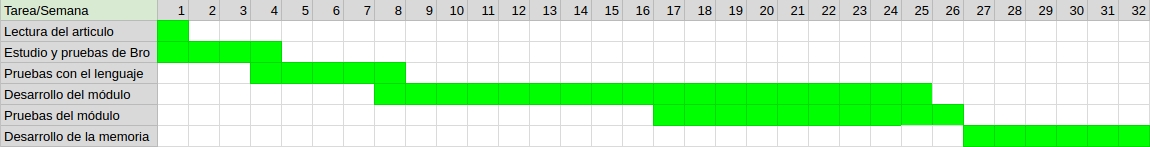
\includegraphics[width=1\textwidth]{imagenes/temporizacion.png} 
  \centering
  \caption{Temporización en diagrama de Gantt.}
\end{figure}

El gasto que requiere este proyecto se desglosa de la siguiente manera.
\begin{itemize}
\item \textit{Licencias}. El gasto en licencias será nulo, pues Bro está creado bajo licencia de software libre \cite{broindex}. El 
módulo será subido a GitHub \cite{repo} con licencia de software libre, por lo que cualquiera podrá usarlo o modificarlo en el futuro.
\item \textit{Equipo}. Teniendo en cuenta que la vida útil de un portátil es de unos 4 años y que el desarrollo de este trabajo 
requiere de unos 6 meses, se tendrá que un portátil de gama media-alta de 800\euro generará un gasto de un octavo de la vida útil. Por 
lo tanto será un coste de unos \textit{100\euro}. Hay que tener en cuenta que Bro solo funciona en Linux o Mac OS X 
\cite{brodownload}, por lo que se está hablando de un portátil y no de un Mac, lo cual supondría un mayor gasto.
\item \textit{Programador}. Según se puede comprobar en Internet \cite{tarifa}, el precio por hora de un programador está entre los 
30\euro y los 40\euro, por lo tanto si en el desarrollo del proyecto se ha necesitado de unas 500 horas y dejando el precio en 30\euro 
la hora, el gasto será de \textit{15000\euro}. Aquí el gasto podría ser mayor, pues no solo se necesita un programador, sino además un 
director de proyecto, lo cual subiría más este gasto.
\item \textit{Varios}. Además de los gastos ya descritos habrá que sumarle una parte de gastos varios como Internet, luz, agua, y 
demás. Unos 150\euro al mes, que al ser 6 meses supone un gasto de \textit{900\euro}.
\end{itemize}

\intro Teniendo en cuenta todos estos cálculos, se tiene que el coste total del proyecto es de unos \textit{16000\euro} por 6 meses de 
trabajo.

\section{Estructura de la memoria}

Esta memoria se organizará de la siguiente forma: 
\begin{itemize}
\item En el capítulo 2 se hablará de todos los fundamentos teóricos y tecnológicos sobre los que se 
basa el proyecto.
\item En el capítulo 3 se contará cómo se pretende resolver el problema expuesto.
\item En el capítulo 4 se encontrará detallado cómo se han implementado los diferentes módulos.
\item En el capítulo 5 se realizarán las pruebas, para comprobar que todo funciona como 
estaba previsto, tanto a nivel funcional como a nivel de aplicación.
\item En el último capítulo se hablará de las conclusiones recogidas a lo largo de este proyecto y las posibles 
opciones que tiene para seguir trabajando sobre él.
\end{itemize}
